\documentclass[
  11pt,
  letterpaper,
   addpoints,
   answers
  ]{exam}

\usepackage{../exercise-preamble}

\begin{document}

\noindent
\begin{minipage}{0.47\textwidth}

\includegraphics[width=\textwidth]{../fcfm_die}
\end{minipage}
\begin{minipage}{0.53\textwidth}
\begin{center} 
\large\textbf{Fundamentos de control de sistemas} (EL4111-1) \\
\large\textbf{Clase auxiliar 4} \\
\small Prof.~Roberto Cardenas Dobson\\
\small Prof.~Aux.~Osvaldo Jimenez - Erik Sáez\\
\small Ayudantes.~Simon Arenas- Juan Pablo Baez - Francisco Garces - Sofia Ibarra\\
\end{center}
\end{minipage}

\vspace{0.5cm}
\noindent
\vspace{.85cm}

\begin{questions}
    %%%%%%%%%%%%%%%%%%%%%%%%%%%
    \question Para la siguiente planta
    \begin{align}
        G_p(s)=\frac{3}{(s+5)(s-5)}
    \end{align}
    Se desea diseñar un controlador que cumpla con un requerimiento de $\omega_n = 15 \text{ rad/seg}$, amortiguación de 0.707, cero error en estado estacionario para entrada escalón y, por razones de costo, debe estar conformado por 2 mallas lead/lag (en cualquiera de sus combinaciones).
    \begin{enumerate}
        \item Todo lo anterior en consideración, encuentre la forma del controlador sabiendo que uno de los elementos de una de las mallas realiza cancelación. Y que casi no existe ruido a alta frecuencia (se permite que el polo de una de las mallas de compensación esté a una distancia 30 veces la frecuencia natural). Justifique cada uno de los elementos que conforman el controlador.
        \item  Calcule la ganancia mínima del controlador calculado en a) para que el sistema se mantenga estable.
        \item Determine el tiempo de establecimiento (2\%) y sobrepaso y también determínelos de manera algebraica. Comente.
    \end{enumerate}
%%%%%%%%%%%%%%%%%%%%%%%%%%%
\begin{solution}
\subsection*{Resolucion 1.1}
Dado que se busca realizar un contorlador con unos requerimientos dados por el enunciado, deberemos recordar la forma de las mallas en atraso o adelanto (lead/lag). Estas mallas tienen la siguiente forma general:
\subsubsection*{Malla en adelanto (lead):}
Se tiene que la malla vendra dada por:
\begin{equation}
    G_{lead}(s)=K\frac{s+a}{s+b}
\end{equation}
Donde el polo estara \textbf{adelantado} con respecto al cero, es decir que $a>b$ esto se visualiza en lo siguiente:
\begin{center}
\begin{tikzpicture}
    \draw[->] (-6,0) -- (2,0) node[right] {$\sigma$};
    \draw[->] (0,-3) -- (0,3) node[above] {$j\omega$};

    \draw[blue, thick] (-2,0) circle (0.15) node[below right] {$a$};

    \draw[red, thick] (-4,0) node[below left] {$b$} -- ++(0.2,0.2) -- ++(-0.4,-0.4) ++(0.4,0) -- ++(-0.4,0.4);
\end{tikzpicture}
\end{center}
\subsubsection*{Malla en atraso (lag):}
Por otro lado se tiene que la forma general de la malla viene dada por:
\begin{equation}
    G_{lead}(s)=K\frac{s+a}{s+b}
\end{equation}
Donde el polo estara \textbf{adelantado} con respecto al cero, es decir que $a<b$ esto se visualiza en lo siguiente:
\begin{center}
\begin{tikzpicture}
    \draw[->] (-6,0) -- (2,0) node[right] {$\sigma$};
    \draw[->] (0,-3) -- (0,3) node[above] {$j\omega$};
    \draw[blue, thick] (-4,0) circle (0.15) node[below left] {$a$};

    \draw[red, thick] (-2,0) node[below right] {$b$} -- ++(0.2,0.2) -- ++(-0.4,-0.4) ++(0.4,0) -- ++(-0.4,0.4);
\end{tikzpicture}
\end{center}
Luego se tendra por enunciado se deberan cumplir los siguiente criterios de diseño para el controlador:
\begin{itemize}
    \item $\omega_n=15$ rad/s
    \item $\xi=0.707$
    \item Cero error en estado estacionario
    \item 2 mallas lead/lag
    \item Cancelación de un polo
    \item Polo a una distancia 30 veces la frecuencia natural
\end{itemize}
Considerando todo lo anterior, se plantea el siguiente controlador:
\begin{align}
    G_{c}(s)= k \left(\frac{s+5}{s}\right)\left(\frac{s+a}{s+15\cdot 30}\right)
\end{align}
Donde para la primera malla tenemos que es de la forma $\frac{s+5}{s}$ donde se observa de manera directa que $(a>b)$ lo que corresponde a una malla en adelanto, ademas se cumple la condicion de cero error a estado estacion para una entrada escalon $\frac{1}{s}$,por otro lado se tiene el elemento utilizado para la cancelacion $(s+5)$, donde evidentemente cancelamos el polo de la planta que es positivo, dado que no es recomendable el cancelar un polo inestable $(s-5)$.Por otro lado se tiene que la segunda malla es de la forma $\left(\frac{s+a}{s+15\cdot 30}\right)$ donde se observa que $a<b$ con lo que corresponde a una malla en atraso, donde se cumple por un lado la condicion de tener un polo a una distancia 30 veces la frecuencia natural y por otro lado se tiene que el cero se encuentra en $(s+a)$ lo cual nos permite el sintonizar el controlador,ademas dada la cancelacion realizada anteriormente, ahora este controlador depende unicamente de una variable, con lo que tenemos que la planta y el controlador se ven de la siguiente forma:
\begin{align}
    G_{p}G_{s} &= \left(\frac{3}{(s+5)(s-5)}\right)\cdot \left(k \cdot \frac{(s+5)(s+a)}{s(s+450)}\right)\\
              &= \frac{3k(s+a)}{s(s-5)(s+450)}\\
\end{align}
Luego para cumplir con los requerimientos de diseño se tendra:
\begin{align}
    \cos(\theta) &= 0.707 \\
    \theta = \cos^{-1}(0.707) &= 45^{\circ} \\
\end{align}
Se obtiene el angulo asociado al punto de diseño,y ademas tenemos que $w_{n}=15 rad/s$ es la distancia del origen al punto de diseño, con lo que se tiene el siguiente esquema:
\begin{center}
    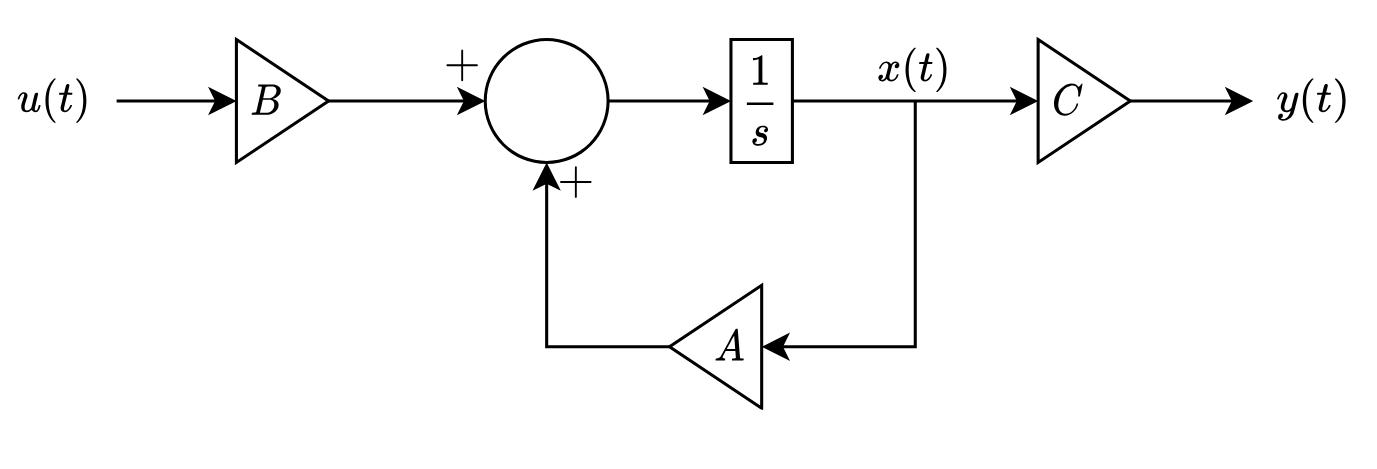
\includegraphics[width=0.6\textwidth]{Auxiliar_4_1}
    \captionof{figure}{Esquema }
\end{center}
Dado que $\theta=45^{\circ}$ podemos hacer uso de pitagoras para poder obtener los lados que son iguales (Notar que es un cuadrado a la mitad),con lo que se tiene que:
\begin{align}
    x^{2} + x^{2} &= 15^{2}\\
    \sqrt{2}x &= 15\\
    x &= 15/\sqrt{2}\\
    x &= 10.6
\end{align}
Con lo que se obtiene que el punto de diseño viene dado por $s_{1,2}=-10.6 \pm j10.6$,luego ubicamos el resto de polos y ceros de la planta:
\begin{center}
    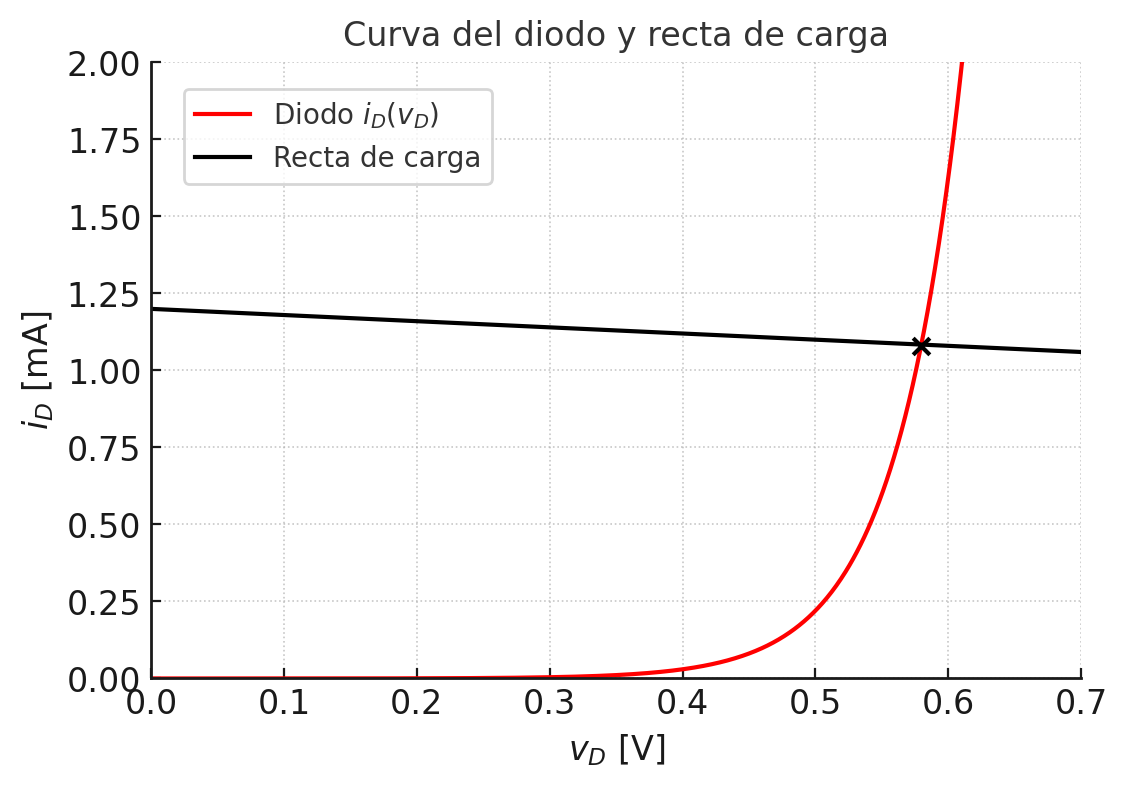
\includegraphics[width=0.7\textwidth]{Auxiliar_4_2}
    \captionof{figure}{LGR de polos y ceros }
\end{center}
Notamos que el $a$ aun es una incognita, por lo aun no sabemos a priori si ubicarlo a la derecha o a la izquierda del punto de diseño. Luego para la condciion de angulo se tiene que:
\begin{align}
    \sum \theta_{i}^{p} - \sum \theta_{i}^{z} &= 180^{\circ}\\
    \theta_{1} + \theta_{2} + \theta_{3} - \theta_{a} &= 180^{\circ}\\
\end{align}
Luego determinamos cada uno de los angulos:
\begin{align}
    \theta_{1} &= \arctan(\frac{10.6}{450-10.6}) = 1.383^{\circ}\\
    \theta_{2} &= 180^{\circ} - \arctan(\frac{10.6}{10.6}) = 135^{\circ}\\
    \theta_{3} &= 180^{\circ} - \arctan(\frac{10.6}{10.6+5})=145.8^{\circ}\\
\end{align}
Con lo que tenemos que el angulo $\theta_{a}$ viene dado por:
\begin{align}
    1.383^{\circ} + 135^{\circ} + 145.8^{\circ} - \theta_{a} &= 180^{\circ}\\
    \theta_{a} &= 102.18^{\circ}
\end{align}
Una vez obtenido el valor del angulo $\theta_{a}$ se tiene que este angulo corresponde a un angulo positivo, con lo que se tiene que el cero se encuentra a la derecha del punto de diseño, con lo que se tiene que el controlador vendra dado por:
\begin{center}
    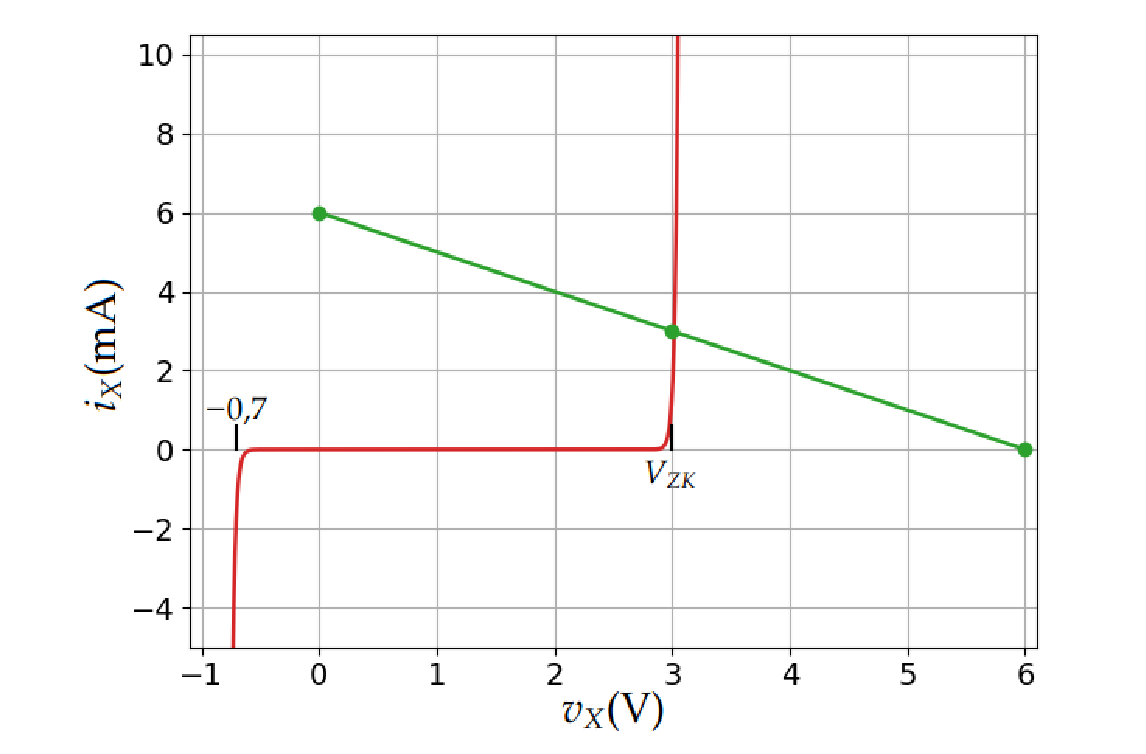
\includegraphics[width=0.6\textwidth]{Auxiliar_4_9}
    \captionof{figure}{LGR con actualizacion de la ubicacion del cero}
\end{center}
Determinamos a por tanto tal que:
\begin{align}
    \theta_{a} = 180 - \arctan(\frac{10.6}{10.6+-a}) &= 102.18\\
    \arctan(\frac{10.6}{10.6-a}) &= 180 - 102.18\\
    \frac{10.6}{10.6-a} &= \tan(77.82)\\
    a &= 8.18
\end{align}
Con lo que se obtiene finalmente la ubicacion del cero,luego debemos obtener la ganancia del controlador,con lo que se tiene que:
\begin{align}
    K &= \abs{\frac{1}{G_{p}(s)G_{c}(s)}}_{s=s^{*}}\\
    K &= \abs{\frac{1}{\frac{3(s+8.18)}{s(s-5)(s+450)}}}_{s=-10.6+j10.6}\\
    K &= 3810.7
\end{align}
Se obtiene la ganancia, por lo que el controlador tendra la siguiente forma:
\begin{align}
    G_{c}(s) = 3810.7\cdot \left(\frac{(s+5)(s+8.18)}{s(s+450)}\right)
\end{align}
No olvidar agregar el termino $(s+5)$ \textbf{en el controlador} en su respuesta final, dado que si bien se cancela con la planta,este debe encontrarse presente en el controlador.
\subsection*{Resolucion 1.2}
Se busca obtener la ganancia minima del controlador para que el sistema se mantenga estable, esto se puede realizar de las formas vistas en auxiliares pasados(Forma geometrica),en particular se utilizara Routhe-Hurwitz,por lo que desarrollando el polinomio se tendra:
\begin{align}
    1+G(s)H(s) = 0\\
    1+G_{p}(s)G_{c}(s) = 0\\
    1+\frac{3k(s+8.18)}{s(s-5)(s+450)} = 0\\
    s(s+450)(s-5 + 3k(s+8.18)) = 0\\
    s^{3} + 445s^{2} - 2250s + 3ks^{2} + 24.54k = 0\\
    s^{3} + 445s^{2} + (3k-2250)s + 24.54k = 0
\end{align}
Con lo que se obtienen los valores de las constantes que seran utilizados para el criterio de estabilidad de Routh-Hurwitz:
\begin{align}
    a_{1} &= 1\\
    a_{2} &= 445\\
    a_{3} &= 3k-2250\\
    a_{4} &= 24.54k
\end{align}
Luego nuestra tabla se vera de la siguiente forma:
\begin{center}
    \begin{tabular}{|c|c|c|}
        \hline
        $s^{3}$ & 1 & (3k-2250)\\
        $s^{2}$ & 445 & 24.54k\\
        $s^{1}$ & $\alpha_{1}$ & $\alpha_{2}$\\
        $s^{0}$ & $\beta_{1}$ & $\beta_{2}$\\
        \hline
    \end{tabular}
\end{center}
Luego recordando lo visto en el auxiliar 2, se tendra que:
\begin{align}
    \alpha_{1} &= \frac{445(3k-2250) - 24.54k}{445}\\
               &= 2.94k - 2250\\
    \alpha_{2} &= 0\\
    \beta_{1}  &= \frac{\alpha_{1} \cdot 24.54k - \alpha_{2}\cdot 445}{\alpha_{1}}\\
               &= 25.54k\\
    \beta_{2}  &=0
\end{align}
Por lo tanto, para sea estable no debe existir un cambio de signo,eso implica que se debe cumplir que $\alpha_{1}>1$ y $\beta_{1}>0$,por lo que se tiene que para $\alpha_{1}$:
\begin{align}
    2.94k - 2250 &> 0\\
    2.94k &> 2250\\
    k &> 765.3
\end{align}
por otro lado para $\beta_{1}$ se tiene que:
\begin{align}
    25.54k &> 0\\
    k &> 0
\end{align}
Se cumple que cuando $k>765.3$ el sistema se mantiene estable,por lo que implica que el caso critico se cumple cuando $k=765.3$.
\subsection*{Resolucion 1.3}
Dado que nos interesa obtener el sobrepaso y el tiempo de establecimiento(2\%) tenemos que:
\begin{align}
    t_{s} &= \frac{4}{\xi \omega_{n}}\\
          &= \frac{4}{0.707\cdot 15}\\
          &= 0.377 s
\end{align}
Luego para el sobrepaso:
\begin{align}
    M_{p} &= 100 \cdot e^{-\frac{\xi \pi}{\sqrt{1-\xi^{2}}}}\\
          &= 100 \cdot e^{-\frac{0.707 \pi}{\sqrt{1-0.707^{2}}} }\\
          &= 4.325 \%
\end{align}
Con lo que se obtiene lo pedido.
\end{solution}
    %%%%%%%%%%%%%%%%%%%%%%%%%%%
    %%%%%%%%%%%%%%%%%%%%%%%%%%%
    \question Considere el diagrama de bloques del sistema indicado por la figura que se muestra a continuación:
    \begin{center}
        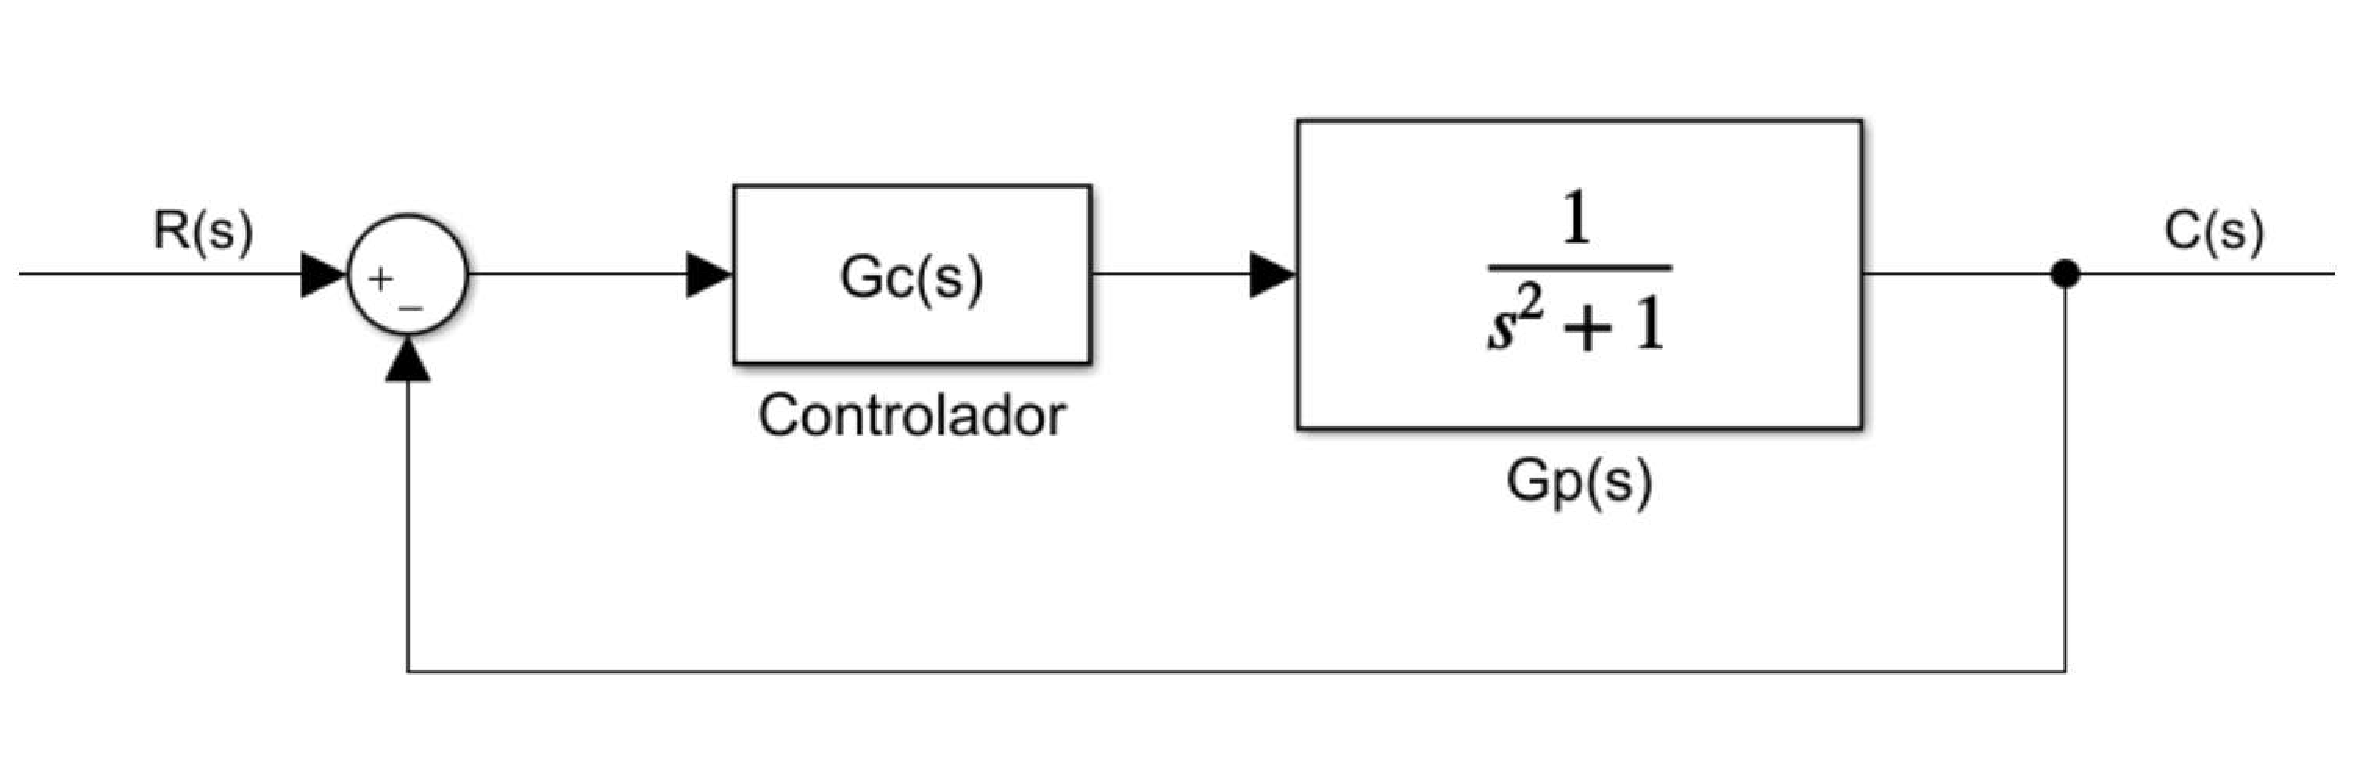
\includegraphics[width=0.7\textwidth]{Auxiliar_4_8}
        \captionof{figure}{Esquema }
    \end{center}
    \begin{enumerate}
    \item Diseñe un controlador PID [Gc(s)] propio e implementable, para la planta Gp(s) utilizando los criterios del módulo y ángulo del lugar de la raíz de forma que se cumplan las siguientes especificaciones:
    \begin{itemize}
        \item Uno de los ceros esté ubicado en $a=-0.8$
        \item Cero error en estado estacionario
        \item El diseño debe ubicar polos de lazo cerrado complejos que se encuentren en los puntos $s = -1 \pm j\sqrt{3}$
    \end{itemize}
    El resto de los elementos del PID deben ser ubicados de forma de minimizar la separación entre el cero y el polo restantes (bisectriz). \textbf{Recuerde.} En este ejercicio es necesario dibujar el posible lugar de la raíz del sistema resultante después de agregar el compensador.
        \item  ¿Cuáles son el tiempo de establecimiento y sobrepaso que cumplen los polos de lazo cerrado? 
        \item ¿Existen más polos de lazo cerrado? de ser así ¿cuántos más son y proponga una metodología o ecuaciones que permitan obtener su posición. 
        \item ¿Existe algún valor de ganancia K, en el compensador, donde el sistema se vuelva inestable? Fundamente de forma gráfica y teórica su respuesta. Utilice el lugar geométrico de la raíz y el criterio de Routh-Hurwitz para resolver esta pregunta. 
        \item Explique ventajas y desventajas de cada controlador creado para la planta G(s)
    \end{enumerate}

%%%%%%%%%%%%%%%%%%%%%%%%%%%
\begin{solution}
\subsection*{Resolucion 2.1}
Se busca realizar un controlador PID para que la planta cumpla los siguientes requerimientos:
\begin{itemize}
    \item Cero error en estado estacionario
    \item Un cero en $a=-0.8$
    \item Polos en $s=-1\pm j\sqrt{3}$
\end{itemize}
Tomando en consideracion lo anterior,se tendra la siguiente estructura para el PID:
\begin{align}
    G_{c}(s) = k \left(\frac{s+0.8}{s}\right)\cdot \left(\frac{s+b}{s+c}\right)
\end{align}
A diferencia de la pregunta anterior, se tendra que no es posible utilizar cancelar algun termino de la planta,por lo que deberemos determinar los valores de $b$ y $c$ tal que minimicen la separacion entre si para mejorar la respuesta,el metodo de la bisectriz da solucion a este problema.Para encontrar el angulo de interes,debemos satisfacer la condicion de angulo.,notamos que la planta se tienen dos polos dados por $p_{1}=j$ y $p_{2}=-j$,luego ubicando el resto de polos y ceros del controlador:
\begin{center}
    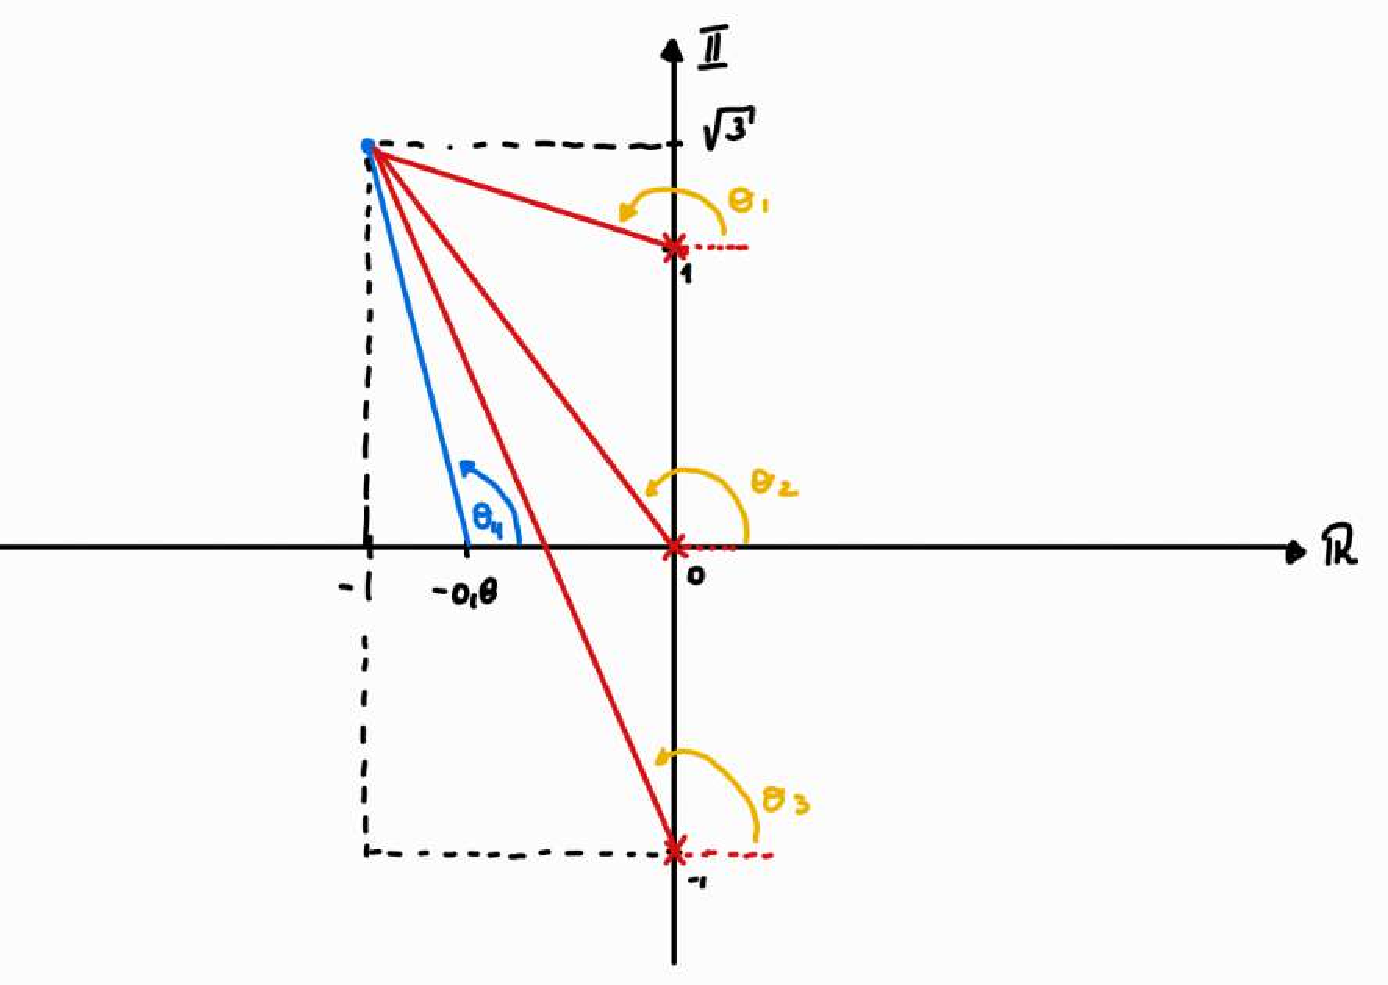
\includegraphics[width=0.6\textwidth]{Auxiliar_4_3}
    \captionof{figure}{Esquema }
\end{center}
Por condicion de angulo tenemos que se debe cumplir:
\begin{align}
    \theta_{1} &= 180 - atan\left(\frac{\sqrt{3}-1}{1}\right) = 143.79^{\circ} \\
    \theta_{2} &= 180 - atan\left(\frac{\sqrt{3}}{1}\right) = 120^{\circ} \\
    \theta_{3} &= 180 - atan\left(\frac{\sqrt{3}+1}{1}\right) = 110.10^{\circ} \\
    \theta_{4} &= 180 - atan\left(\frac{\sqrt{3}}{1-0.8}\right) = 96.59^{\circ}
\end{align}
Luego tendremos que determinar el angulo $\theta_{c}$ y $\theta_{b}$(Que corresponden a el cero y polo de nuestro controlador PID a sintonizar),por lo se adiciona a la condicion de angulo como un $\Delta\theta$,tal que:
\begin{align}
    \theta_{1} + \theta_{2} + \theta_{3} - \theta_{4} -\Delta\theta &= 180^{\circ}\\
    \Delta\theta = 97.3^{\circ}
\end{align}
Es imoprtante que el angulo $\Delta\theta$ se reste, dado que estamos realizando una compensación.Luego para aplciar el metodo de la bisectriz aplicaremos la sigueinte metodologia (\textit{Recomiendo revisar el apunte donde se deriva mas en detalle}):
\begin{enumerate}
    \item Desde el punto de diseño se traza una horizontal y un rayo hacia el origen
    \begin{center}
        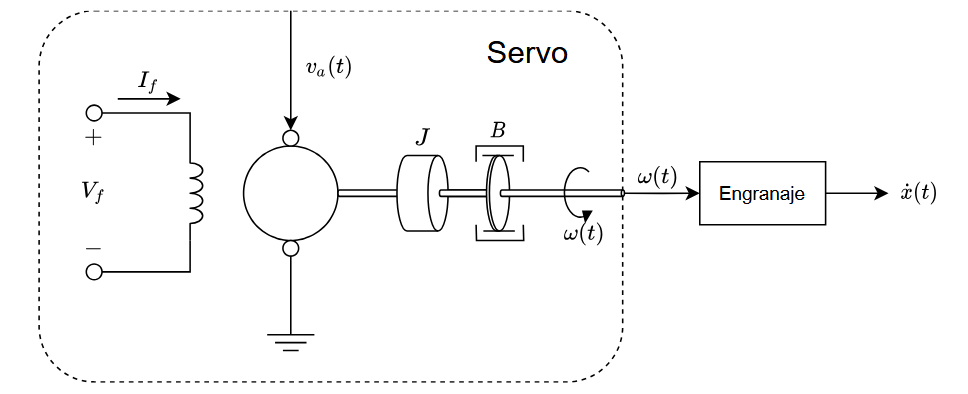
\includegraphics[width=0.6\textwidth]{Auxiliar_4_4}
        \captionof{figure}{Esquema }
    \end{center}
    \item Luego se traza la bisectriz de dicha interseccion.
    \begin{center}
        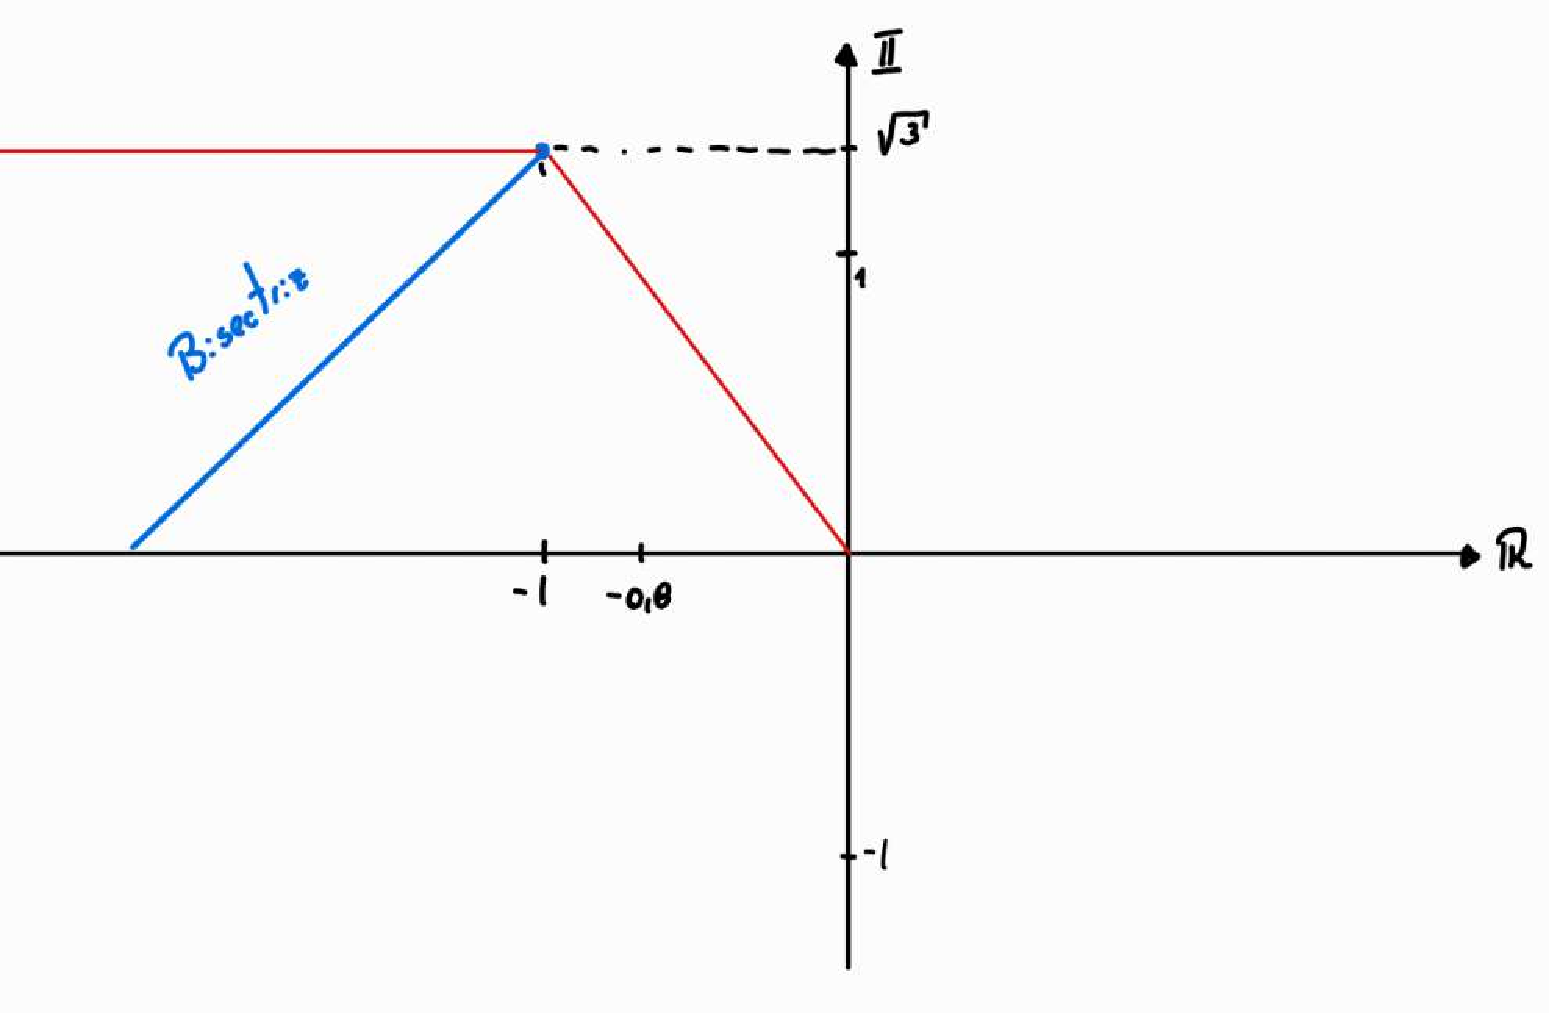
\includegraphics[width=0.6\textwidth]{Auxiliar_4_5}
        \captionof{figure}{Esquema }
    \end{center}
    \item Luego debemos abrir un angulo de $\Delta\Theta/2$, con lo que se obtiene el siguiente esquema:
    \begin{center}
        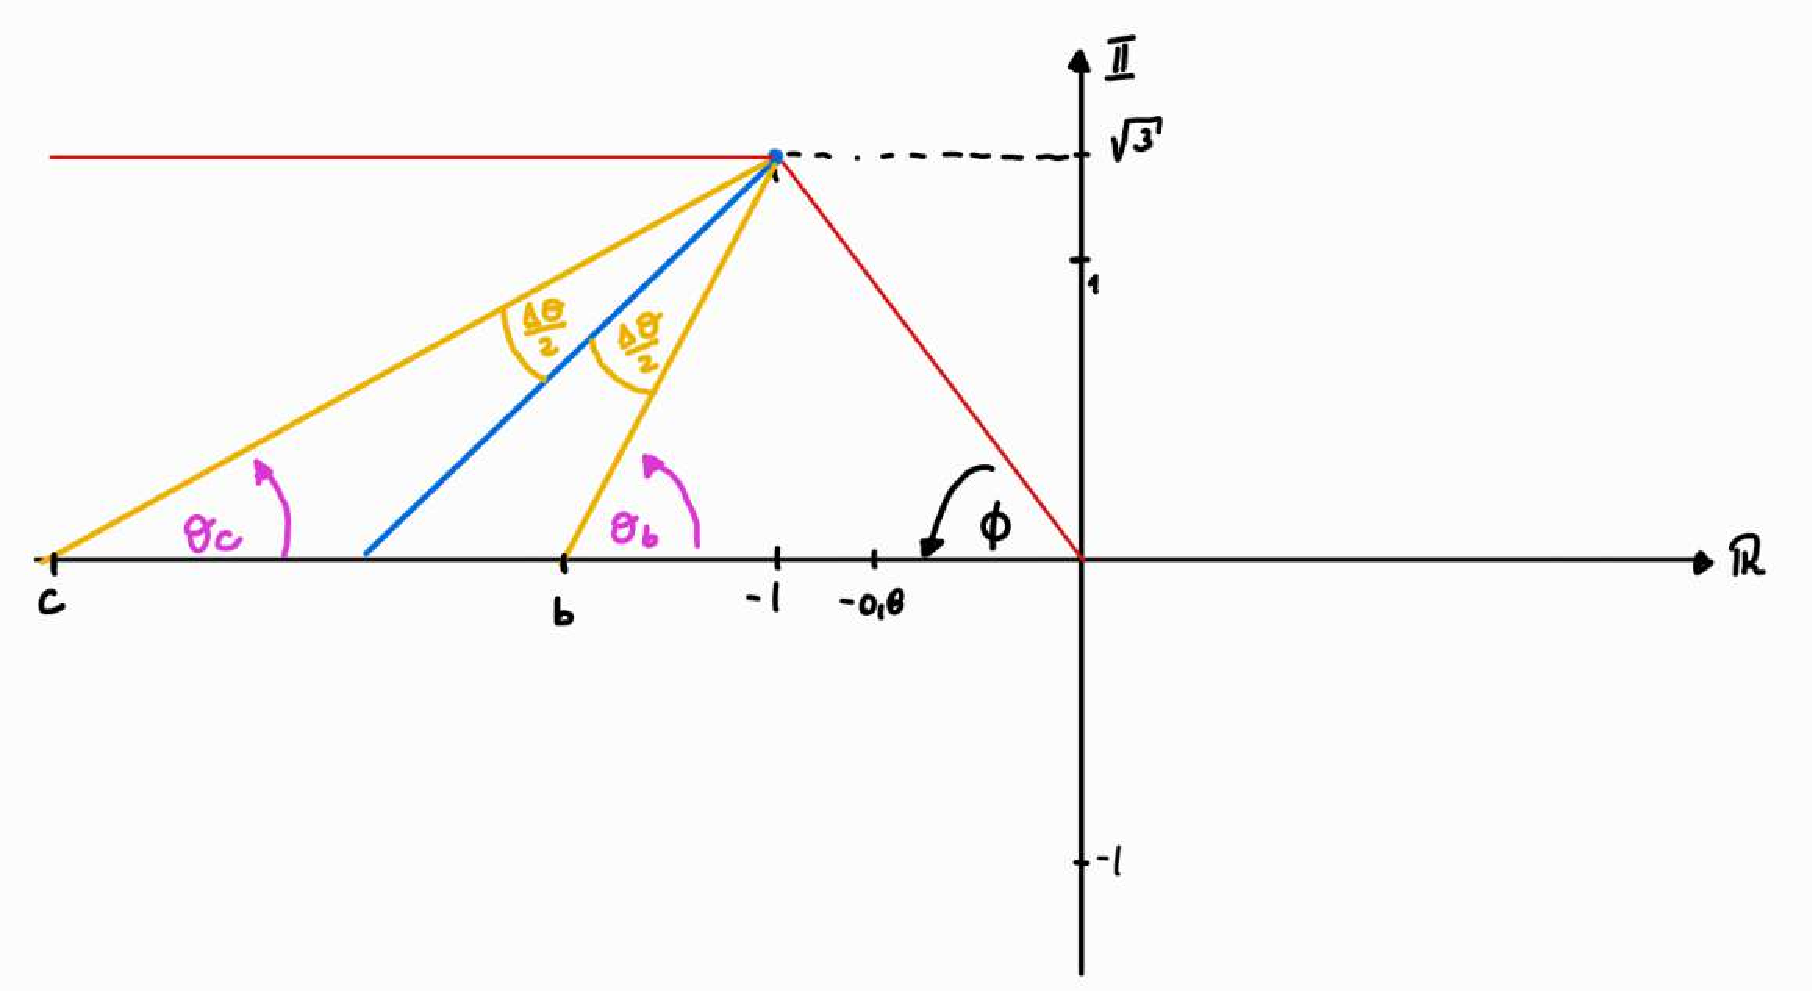
\includegraphics[width=0.7\textwidth]{Auxiliar_4_6}
        \captionof{figure}{Esquema }
    \end{center}
\end{enumerate}
De esta manera se identifican los angulos que son de interes,se puede demostrar geoemtricamente que:
\begin{align}
    \theta_{c} &= 90 - \frac{\phi}{2} - \frac{\Delta \theta}{2}\\ 
    \theta_{b} &= 90 + \frac{\phi}{2} - \frac{\Delta \theta}{2}
\end{align}
Donde se obtiene el angulo $\phi$ tal que:
\begin{align}
    \phi = 180^{\circ} - 120^{\circ} = 60^{\circ}
\end{align}
Con lo que tenemos que $\theta_{c}$ y $\theta_{b}$ vendran dado por:
\begin{align}
    \theta_{c} &= 90 - \frac{60}{2} - \frac{97.3}{2} = 11.35^{\circ}\\
    \theta_{b} &= 90 - \frac{60}{2} + \frac{97.3}{2} = 108.65^{\circ}
\end{align}
Luego tenemos que el angulo $\theta_{b}>90^{\circ}$ con lo que tendremos que ubicarlo a la derecha del punto de diseño:
\begin{center}
    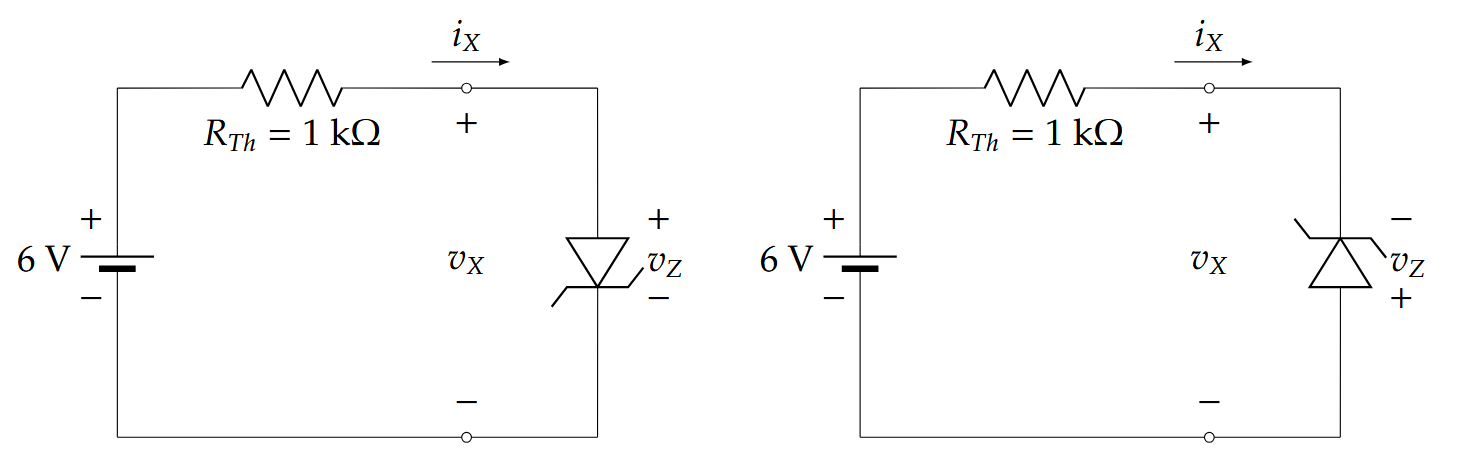
\includegraphics[width=0.7\textwidth]{Auxiliar_4_7}
    \captionof{figure}{Esquema }
\end{center}
De esta manera tenemos que los valores de b y c deberan ser:
\begin{align}
    \theta_{b}=108.65^{\circ}&= 180 - atan(\frac{\sqrt{3}}{1-b})\\
    b&= 0.42\\
    \theta_{c}= 11.35^{\circ} &= atan(\frac{\sqrt{3}}{c-1})\\
    &=9.63
\end{align}
La forma del controlador PID vendra dada por:
\begin{align}
    G_{c} = k\cdot \frac{(s+8)}{s}\left(\frac{s+0.42}{s+9.63}\right)
\end{align}
Luego determinamos la ganancia del controlador como:
\begin{align}
    K &= \abs{\frac{1}{G_{p}(s)G_{c}(s)}}_{s=s^{*}}\\
    K &= \abs{\frac{1}{\frac{1}{s(s^{2}+1)}\frac{(s+0.8)(s+0.42)}{(s+9.63)}}}_{s=-1+j\sqrt{3}}\\
    K &= 19.93
\end{align}
De esta manera tenemos que el controlador PID vendra dado por:
\begin{align}
    G_{c} = 19.93\cdot \frac{(s+0.8)(s+0.42)}{s(s+9.63)}
\end{align}
\subsection*{Resolucion 2.2}
Se busca obtener el tiempo de establecimiento y el sobrepaso de los polos de lazo cerrado,para esto necesitamos obtener $\xi$ y $w_{n}$,los cuales ya fueron obtenidos con anterioridad.Otra forma de obtenerlos es que los polos sintonizados deberan cumplir con la ecuacion de los polos de segundo orden ideal, es decir:
\begin{align}
    s^{2}+ 2\xi w_{n}s + w_{n}^{2} = 0\\
\end{align}
Por lo que tenemos que para el punto de diseño:
\begin{align}
    (s+1+j\sqrt{3})(s+1-j\sqrt{3}) &= s^{2} + 2s + 4\\
\end{align}
Con lo que tenemos que $w_{n}^{2}=4$ con lo que $w_{n}=2$ y para el otro termino tenemos que $2\xi w_{n} = 2$ con lo que $\xi = 0.5$,luego se tiene que:
\begin{align}
    t_{s} &= \frac{4}{\xi w_{n}}\\
          &= \frac{4}{0.5\cdot 2}\\
          &= 4 s
\end{align}
\begin{align}
    M_{p} &= 100 \cdot e^{-\frac{\xi \pi}{\sqrt{1-\xi^{2}}}}\\
          &= 100 \cdot e^{-\frac{0.5 \pi}{\sqrt{1-0.5^{2}}} }\\
          &= 16.30 \%
\end{align}
\subsection*{Resolucion 2.3}
Para responder esta pregunta,debemos recordar que todo el analisis que se realizo fueron para solo dos polos,y que debemos tener la misma cantidad de polos abiertos que de lazo cerrado,ademas de que el modelo que ralizamos para encontrar el LGR es para sistemas de segundo orden ideal,para encontrar el resto de polos se retomara la ecuacion caracteristicas de los polos de lazo cerrado:
\begin{align}
    1+KG_{c}(s)G_{p}(s) = 0
\end{align}
Reemplazando en base a lo que obtuvimos anteriormente se tiene:
\begin{align}
    1+ 19.93\cdot \frac{(s+0.8)(s+0.42)}{s(s+9.63)}\cdot \frac{1}{(s^{2}+1)} &= 0\\
    (s+9.63)s(s^{2}+1) + 19.93(s+0.8)(s+0.42) &= 0\\
    s^{4} + 9.63s^{3}+20.93s^{2}+33.94s + 6.69=0
\end{align}
De esta manera se obtiene lo siguiente:
\begin{align}
    s_{1} &= -1+j\sqrt{3}\\
    s_{2} &= -1-j\sqrt{3}\\
    s_{3} &= -0.225\\
    s_{4} &= -6.8857 
\end{align}
Con lo que se obtienen los puntos de diseño, ademas del resto de polos que dan cuenta del modelo completo,que en la practica se deben tener en cuenta,en analisis de estabilidad.
\subsection*{Resolucion 2.4}
Se busca analisar si existe algun valor de ganancia K en el compensador, donde el sistema se vuelva inestable,para esto se debe realizar un analisis de estabilidad,por lo que se debe realizar un analisis de Routh-Hurwitz,para esto se tiene que expresar como polinomio, es decir:
\begin{align}
    1+KG_{c}(s)G_{p}(s) &= 0\\
    s(s+9.63)(s^{2}+1) + k(s+0.42)(s+0.963)&=0\\
    s^{4}+9.63s^{3} + (k+1)s^{2} + (1.22k+9.63)s + 0.336k &= 0
\end{align}
Con lo que se obtienen los valores de las constantes que seran utilizados para el criterio de estabilidad de Routh-Hurwitz:
\begin{align}
    \alpha_{4} &= 1\\
    \alpha_{3} &= 9.63\\
    \alpha_{2} &= k+1\\
    \alpha_{1}&= 1.22k+9.63\\
    \alpha_{0}&= 0.336k
\end{align}
Luego nuestra tabla de Routh-Hurwitz se vera de la siguiente forma:
\begin{center}
    \begin{tabular}{|c|c|c|c|}
        \hline
        $s^{4}$ & $\alpha_{4}$ & $\alpha_{2}$  & $\alpha_{0}$ \\
        $s^{3}$ & $\alpha_{3}$ & $\alpha_{1}$  & -\\
        $s^{2}$ & $\beta_{1}$ & $\beta_{2}$  & -\\
        $s^{1}$ & $c_{1}$  & -   & -\\
        $s^{0}$ & $d_{1}$ & -  & - \\
        \hline
    \end{tabular}
\end{center}
reemplazando tenemos que:
\begin{center}
    \begin{tabular}{|c|c|c|c|}
        \hline
        $s^{4}$ & 1  & k+1  & 0.336k \\
        $s^{3}$ & 9.63 & (1.22k+9.63)  & -\\
        $s^{2}$ & $\beta_{1}$ & $\beta_{2}$  & -\\
        $s^{1}$ & $c_{1}$  & -   & -\\
        $s^{0}$ & $d_{1}$ & -  & - \\
        \hline
    \end{tabular}
\end{center}
Luego calculamos los parametros tal que:
\begin{align}
    \beta_{1}&= \frac{9.63(k+1)-(1.22k+9.63)}{9.63}\\
             &=0.87k\\
    \beta_{2}&= \frac{9.63 \cdot 0.336k - 0 \cdot 1}{9.63}\\
             &=0.336k\\
    c_{1} &= \frac{0.87k(1.22k+9.63)-0.336k\cdot 9.63}{0.87k}\\
            &= 1.26k + 5.91\\
    d_{1} &= 0.336k
\end{align}
Asi tenemos que:
\begin{center}
    \begin{tabular}{|c|c|c|c|}
        \hline
        $s^{4}$ & 1  & k+1  & 0.336k \\
        $s^{3}$ & 9.63 & (1.22k+9.63)  & -\\
        $s^{2}$ & 0.87k & 0.336k  & -\\
        $s^{1}$ & 1.26k+5.91  & -   & -\\
        $s^{0}$ & 0.336k & -  & - \\
        \hline
    \end{tabular}
\end{center}
No debe existir cambio de signo se debe cumplir:
\begin{align}
    0.87k &> 0\\
    1.26k + 5.91 &> 0\\
    0.336k &> 0
\end{align}
En conjunto se debe cumplir,que $k>0$ y $k>-4.69$,y dado que consideramos incialmente que la ganancia $k>0$,tenemos que siempre se cumplira la condicion de estabilidad.
\subsection*{Resolucion 2.5}
Buscamos analizar que ventajas tiene implementar un controlador mediante cancelacion y otro mediante Sintonizacion.Para el caso de cancelacion tenemos ventajas claras con respecto al otro,como por ejemplo un menor grado de libertad,pero el problema principal radica en que los polos se pueden mover y por tanto si este se encuentran cerca de alguna zona de inestabilidad se pueden mover levemente los polos y no obtener una cancelacion perfecta.Pero por otro lado el PID tiene la ventaja que limita la accion integral del controlador cuando este se encuentra en saturacion (Lo veremos proximamente),pero su sintonizacion es algo mas compleja al igual que su implementacion.
\end{solution}
%%%%%%%%%%%%%%%%%%%%%%%%%%%
\end{questions}
\newpage
%%%%%%%%%%%%%%%%%%%%%%%%%%%

\end{document}